\documentclass[a4paper,12pt]{article}

\usepackage{hyperref}
\usepackage{graphicx}
\graphicspath{ {./images/} }

\begin{document}

\section{Introduction}

Mathematical formulations for the subcellular metrics computed on MERFISH datasets

\section{Informal description of available data}

MERFISH data from the preprint \href{https://www.biorxiv.org/content/10.1101/2020.06.04.105700v1}{here} has cell-boundary and RNA spot information available for $238,000$ cells with $252$ different genes.
Not all cells have RNA spots detected for all genes.


Cell-boundaries take the form of a list of (x,y) positions for each cell.
Drawing a straight line between each position in this list results in a closed polygon that represents the outside boundary of the cell

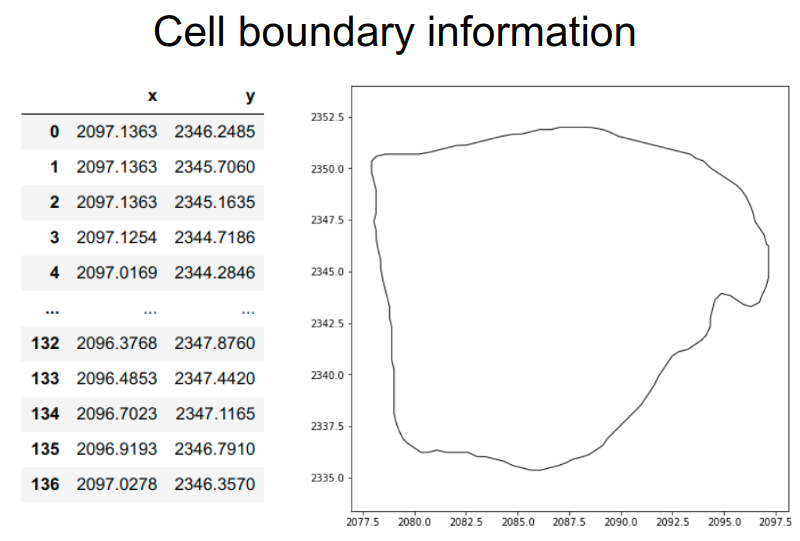
\includegraphics[scale=0.35]{boundary_info.png}


RNA-spots are the MERFISH imaging output and contain information for both x,y location of the spot, and the RNA identity at that location.
I've identified which RNA spots are within each cell boundary.

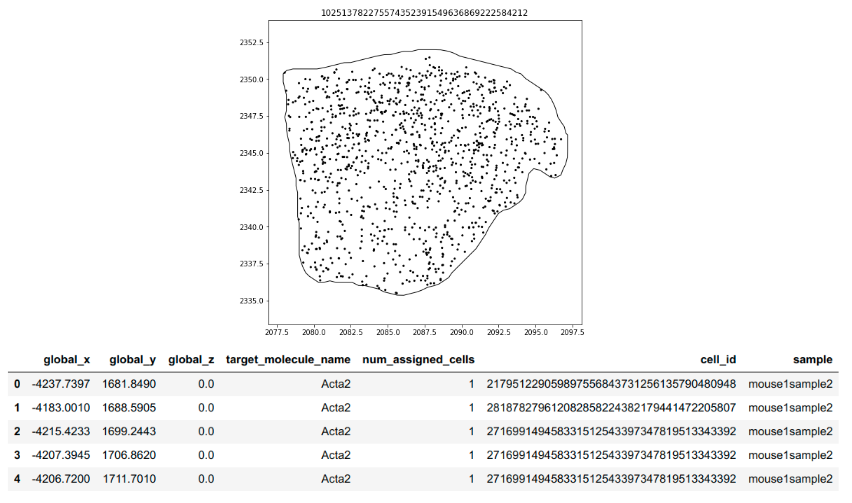
\includegraphics[scale=0.5]{spots_in_cell.png}

\section{Definitions}

There are $n$ spots, $c$ cells, and $g$ unique genes in the total dataset

\begin{itemize}
    \item Let $P$ be a matrix of positions of each RNA spot. $P$ has dimensions of $n$ by 2 for the x and y coordinates

    \item Let $I$ be an binary matrix of size $n$ by $c$, where $I_{i,j} = 1$ indicates that RNA spot $i$ is within cell $j$, and 0 otherwise. Row sums are 1.

    \item Let $G$ be a binary matrix of size $n$ by $g$ where $G_{i,j} = 1$ if RNA spot $n$ is of gene type $G$ and 0 otherwise. Row sums are 1.

    \item Let $X$ be the number of RNA spots per gene per cell, defined by $I^{T}G$. $X_{i,j}$ is the number of RNA spots of gene $j$ in cell $i$. $X$ has dimensions of $c$ by $g$.

    \item Let $Y$ be a binary matrix of size $c$ by $g$ where $Y_{i,j} = 1$ if cell $i$ has at least one RNA spot of gene $g$ and 0 otherwise.

\end{itemize}


From these definitions we can formulate all calculations below

\section{Common calculations}

Count the number of all RNA spots, regardless of gene-type, in cell $c$
\begin{equation}
    \sum_{i=1}^{n} I_{i,c}
\end{equation}


Count the number of RNA spots of type $g$ in cell $c$

\begin{equation}
    \sum_{i=1}^{n} G_{i,g}I_{i,c}
\end{equation}


Count the number of unique genes in cell $c$
\begin{equation}
    \sum_{i=1}^{g} Y_{c,i}
\end{equation}

Get the average x-position of all RNA spots of gene $g$ in cell $c$
\begin{equation}
    \frac{\sum_{i=1}^{n} I_{i,c}G_{i,g}P_{i,1}}{X_{c,g}}
\end{equation}

Get the average y-position of all RNA spots of gene $g$ in cell $c$
\begin{equation}
    \frac{\sum_{i=1}^{n} I_{i,c}G_{i,g}P_{i,2}}{X_{c,g}}
\end{equation}



\section{Metric definition}

All metrics are functions that are applied to each cell/gene pair and result in a scalar value.

Let $M$ be a metric such that $M(c,g)$ is a real number for the result of the metric calculation on gene $g$ in cell $c$. $M(c,g)$ is only defined if there is at least one RNA spot of gene $g$ in cell $c$ ($Y_{c,g} = 1$)

In order to compare the results of metric $M$ between cells with different sizes and shapes, I am Z-score normalizing $M$ over all genes within each cell.

The Z-score normalization for gene $g$ in cell $c$ is defined to be $M(c,g)$ minus the mean of $M$ for cell $c$ over all genes, divided by the variance of $M$ for cell $c$ over all genes.

The mean of $M$ over all genes in cell $c$ is defined as:
\begin{equation}
    Mean(M(c)) = \frac{\sum_{i=1}^{g}M(c,i)}{\sum_{i=1}^{g}Y_{c,i}}
\end{equation}

The var of $M$ over all genes in cell $c$ is defined as:
\begin{equation}
    Var(M(c)) = \frac{\sum_{i=1}^{g}(M(c,i)-Mean(M(c)))^{2}}{(\sum_{i=1}^{g}Y_{c,i})-1}
\end{equation}

Then finally we have the definition for the Z-normalized metric on gene $g$ for cell $c$
\begin{equation}
    Z(c,g) = \frac{M(c,g)-Mean(M(c))}{Var(M(c))}
\end{equation}


\section{Centrality metric}

This metric calculates the mean distance of all the RNA spots of gene $g$ in cell $c$ from the cell centroid.

For this metric we will make a new definition for the cell centroids

\begin{itemize}
    \item Let $C$ be cell centroids where $C_{i,1}$ is the x-centroid location of cell $i$. $C_{i,2}$ is the y-centroid location. $C$ has shape $c$ by $2$
\end{itemize}

Then lets define a distance function $D(i,j)$ to be the L2 distance between the centroid of cell $i$ and the position of RNA spot $j$
\begin{equation}
    D(i,j) = \sqrt[]{(C_{i,1}-P_{j,1})^{2}+(C_{i,2}-P_{j,2})^{2}}
\end{equation}

\begin{equation}
    M_{centrality}(c,g) = \frac{\sum_{i=1}^{n}D(c,i)I_{i,c}}{X_{c,g}}
\end{equation}

\section{Polarity metric}

\section{Periphery metric}

\end{document}

